\scanpage{26}
Alors $Z,Z'$ ont des images inverses $Z_1,Z'_1$ sur $X\times T_1$, et si $\nu,\nu'$ sont les $0$-cycles de $T,T'$ comme dans 1.1., on peut les remonter en $\nu_1=\nu\times a'$, $\nu'_1=a\times\nu'$ de $T\times T'$. Notons que
\[
S_{T\times T'}(\nu\times a')=S_{\unsure{Y|T}}(\nu)=0,\quad S_{T\times T'}(a\times\nu')=S_{T'}(\nu')=0
\]
\margin{\figure{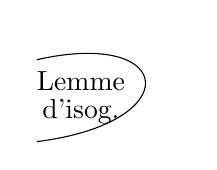
\begin{tikzpicture}[scale=.8]
\node at (0,0) {\shortstack{\unsure{Lemme}\\\unsure{d'isog.}}};
\draw (-.7,.6) .. controls (1.5,1.1) and (1.7,-.4) .. (-.7,-.7);
\end{tikzpicture}}}
donc $\nu_1^{\unsure{*}}$ et $\nu'_1$ sont \deleted{Alb-équi.} \inserted{de degré $0$ et} tels que les $S_{T\times T'}$ sont nuls. D'autre part, on voit de suite que
\[
Z_1(\nu_1)=Z(\nu),\quad Z'(\nu'_1)=Z'(\nu'),
\]
\deleted{donc on est} d'autre part
\[
Z_1(\nu'_1)=Z(\operatorname{pr}_{1*}(\nu'_1))=0
\]
car $\operatorname{pr}_{1*}(\nu'_1)=0$, sous réserve que $Z$ a été choisi tel que $Z(a)$ soit défini. On a de $=$, si $a'$ est choisi convenablement, $Z'_1(\nu_1)=0$.

On pose donc
\[
Z_2=Z_1+Z'_1,\qquad\nu_2=\nu_1+\nu'_1,
\]
et on aura
\[
Z_2(\nu_2)=z+z'.
\]
\deleted{\unsure{et}} Donc $N(X)$ est bien un \unsure{k-groupe|s-groupe} de $X$.

\margin{\diagram{\begin{tikzcd}[ampersand replacement=\&]
X\times T\arrow[d,dash] \& X\times T\times T'\arrow[l,dash]\arrow[d,dash]\\
T \& T\times T'\arrow[l,dash]
\end{tikzcd}}}

\mspage{25}
